\documentclass[a4paper,12pt]{article}
\usepackage[utf8]{inputenc}

\usepackage[utf8]{inputenc}
\usepackage[T2A]{fontenc}
\usepackage[english,russian]{babel}
\usepackage{amsthm}
\usepackage{amsmath}
\usepackage{amssymb}
\usepackage{tikz}
\usepackage{textcomp}
\usepackage{marvosym}
\usepackage{ esint }
\usepackage{mathtext}
\usepackage{siunitx} % Required for alignment
\usepackage{subfigure}
\usepackage{multirow}
\usepackage{rotating}
\usepackage{afterpage}
\usepackage[arrowdel]{physics}
\usepackage{booktabs}
\setlength{\topmargin}{-0.5in}
\setlength{\textheight}{9.1in}
\setlength{\oddsidemargin}{-0.4in}
\setlength{\evensidemargin}{-0.4in}
\setlength{\textwidth}{7in}
\setlength{\parindent}{0ex}
\setlength{\parskip}{1ex}
\newcommand{\ndiv}{\hspace{-4pt}\not|\hspace{2pt}}
\usepackage{graphicx}
\usepackage{float}
\usepackage{wrapfig}
\usepackage{pgfplots}
\usepackage{caption}
\pgfplotsset{compat=1.16}
\graphicspath{ {./images/} }
\usepackage{graphicx}
\RequirePackage{caption}
\DeclareCaptionLabelSeparator{defffis}{ — }
\captionsetup{justification=centering,labelsep=defffis}
\usepackage{caption} \captionsetup[table]{labelsep=endash,justification=justified,singlelinecheck=false,font=normalsize}
\usepackage{amsfonts,mathtools}

\title{Лабораторная работа № 5.1.2\\Исследование эффекта Комптона}
\author{Илья Прамский}
\date{Сентябрь 2024}

\begin{document}
\maketitle
\newpage
\section{Теоретическая справка}
Рассмотрим взаимодействие фотона и электрона, как упругое соударение двух частиц. Запишем для рассматриваемого процесса законы сохранения энергии и импульса:

\[mc^2 + \hbar \omega_0 = \gamma mc^2 + \hbar \omega_1\]

\begin{equation}
\frac{\hbar \omega_0}{c} = \gamma mv \cos{\varphi} + \frac{\hbar \omega_1}{c} \cos{\theta}
\end{equation}
\[\gamma mv \sin{\varphi} = \frac{\hbar \omega_1}{c} \sin{\theta}\]

Перейдя к длинам волн $\lambda_0$ и $\lambda_1$, получим изменение длины волны рассеянного излучения:
\begin{equation}
\Delta \lambda = \lambda_1 - \lambda_0 = \frac{h}{mc} (1 - \cos{\theta}) = \Lambda_k (1 - \cos{\theta})
\end{equation}
Где $\Lambda_k = \frac{h}{mc} = 2,42 \cdot 10^{-10}$ см - комптоновская длина волны электрона.

В дальнейшем же будет удобнее пользоваться другим видом полученной формулы:
\begin{equation}
\frac{1}{\varepsilon(\theta)} - \frac{1}{\varepsilon_0} = 1 - \cos{\theta}
\end{equation}
где $\varepsilon_0 = \frac{E_0}{mc^2}$ - начальная энергия $\gamma$-квантов в единицах $mc^2$, $\varepsilon(\theta)$ - энергия рассеянных $\gamma$-квантов в тех же единицах.

Схема экспериментальной установки:

\begin{figure}[H]
\centering
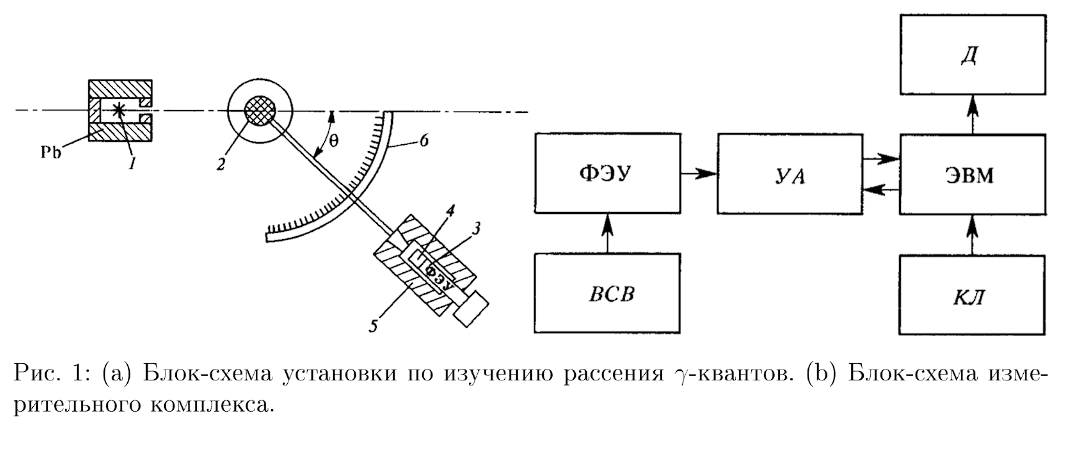
\includegraphics[scale=0.7]{scheme.png}
\end{figure}

Воспользуемся также тем, что $\varepsilon(\theta) = A N(\theta)$, где $N(\theta)$ - номер канала, соответствующего вершине фотопика при данном $\theta$, A - коэффициент пропорциональности. Тогда формулу (3) можно переписать в другом виде:
\begin{equation}
\frac{1}{N(\theta)} - \frac{1}{N(0)} = A(1-\cos{theta})
\end{equation}
Тогда энергию покоя электрона можно определить как:
\begin{equation}
mc^2 = E_\gamma \frac{N(90)}{N(0) - N(90)}
\end{equation}
Где $E_\gamma = E(0)$ - энергия $\gamma$-лучей, испускаемых источником(в нашем случае $^{137}Cs$.
\section{Ход работы}
По измеренным данным составим таблицу и построим график зависимости $\frac{1}{N(\theta)} = f(1-\cos{\theta})$.

\begin{table}[H]
\begin{tabular}{|c|c|c|c|c|c|c|c|c|c|c|c|c|}
\hline
$\theta, ^{\circ}$ & 0 & 10 & 20 & 30 & 40 & 50 & 60 & 70 & 80 & 90 & 100 & 110 \\
\hline
$1-\cos{\theta}$ & 0 & 0,015 & 0,060 & 0,134 & 0,234 & 0,357 & 0,500 & 0,658 & 0,826 & 1,000 & 1,174 & 1,342 \\
\hline
$N$ & 846 & 820 & 754 & 707 & 645 & 582 & 468 & 460 & 416 & 383 & 344 & 315 \\
\hline
$\sigma_N$ & 11 & 7 & 11 & 17 & 38 & 21 & 27 & 19 & 22 & 18 & 14 & 13 \\  
\hline
$\frac{1}{N}, 10^{-3}$ & 1,18 & 1,22 & 1,33 & 1,41 & 1,55 & 1,72 & 2,14 & 2,17 & 2,40 & 2,61 & 2,90 & 3,17 \\
\hline
$\sigma_{\frac{1}{N}}, 10^{-3}$ & 0,02 & 0,01 & 0,02 & 0,03 & 0,09 & 0,06 & 0,12 & 0,09 & 0,13 & 0,12 & 0,11 & 0,13  \\
\hline


\end{tabular}
\end{table}

\begin{figure}[H]
\centering
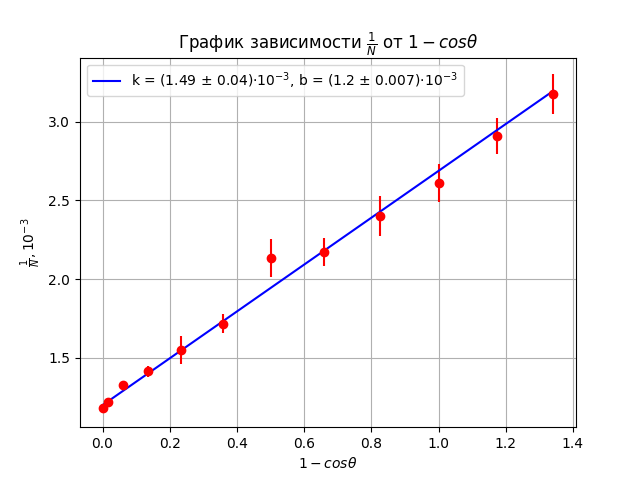
\includegraphics[scale=1]{graph.png}
\end{figure}
Из графика получается
\[A = (1,49 \pm 0,04) \cdot 10^{-3}\]

\[\frac{1}{N_\text{наил}(0)} = (1,200 \pm 0,007) \cdot 10^{-3}\]
Теперь найдём $N_\text{наил}(0)$ и $N_\text{наил}(90)$, используя данные значения.

$N_\text{наил}(0) = 833 \pm 5$
\[N_\text{наил}(90) = \frac{1}{\frac{1}{N_\text{наил}(0)} + A} = 372 \pm 6\]
Получается энергия покоя электрона(учитывая, что $E_\gamma = 662$ кэВ, по формуле (5)).
\[mc^2 = 534 \pm 16 \text{кэВ}\]

\section{Вывод}
В ходе данной работы была оценена энергия покоя электрона, она получилось равной $mc^2_\text{эксп} = 534 \pm 16$ кэВ, теоретическое же значение $mc^2_\text{теор} = 511$ кэВ.
\end{document}